% Chapter 3

\chapter{Geometric Active Contours} % Main chapter title

\label{GAC_chapter} % For referencing the chapter elsewhere, use \ref{Chapter2} 

\lhead{Chapter 4. \emph{Geometric Active Contours}} % This is for the header on each page - perhaps a shortened title

%----------------------------------------------------------------------------------------

Object detection and image segmentation are arguably one of the more investigated fields in computer vision and image analysis. Although in certain cases the terms detection and segmentation are used almost synonymously, there exists subtle differences between them; an object detection algorithm can be deemed successful if it can effectively determine and localize the object of interest in the image. Segmentation, however, requires further analysis. Here we are more concerned with the morphological properties of the object such as shape, connectivity etc. and therefore, a crude detection is not always sufficient. One may think of object detection as the first step for segmentation. In fact, many segmentation methods allow the user to perform an initial detection, either automatically or semi-automatically. The segmentation algorithm then starts from the initialized position and eventually converges when the object boundaries are captured.

Active contour based methods (a.k.a. \textit{snakes}) fall under the category of segmentation algorithms which assume the image to be a  continuously differentiable function. The basic reason for this continuous domain modeling is that the mathematical formulation can be done with the help of continuous domain calculus, which is remarkably strong and well established. The continuous model is eventually discretized, borrowing tools from numerical analysis for practical implementation.

\section{Framework for contour propagation}

Let $f(\textbf{x}):\Omega\mapsto\mathbb{R}$ be a continuous image function, $\forall\textbf{x}\in\Omega$. Traditionally, the domain $\Omega\subseteq\mathbb{R}^2$ or  $\Omega\subset\mathbb{R}^3$ for 2D or 3D cases respectively. In the 3D case, we have \textit{active surfaces} instead of contours and the formulations are modified accordingly. However, most of the mathematics and models are consistent between 2D and 3D applications and therefore, for the sake of simplicity, we will restrict ourselves to the 2D case for basic analysis in this chapter. In the next chapter, where we introduce an explicit 3D model, we will discuss the theories for the 3D case separately.

Considering we have a 2D image $f(\textbf{x}),\;\textbf{x}=(x,y)\in\Omega\subseteq\mathbb{R}^2$, we define a parametric curve $\textbf{C}(p)=\{\textbf{x}(p)\}$, where the parameter $p\in\left[0,1\right]$. To perform segmentation, an initial contour is deformed under the influence of a force field. Mathematically, one can write the curve evolution equation as $\textbf{C}_t(p)=\textbf{F}$. Here $\textbf{F}$ is the \textit{curve velocity}, which is also known as \textit{force vector}. Decomposing the velocity in the normal and tangential direction, we derive the general curve evolution equation as follows:
\bea
\textbf{C}_t(p) = F_n(p)\textbf{n}(p)+F_t(p)\textbf{t}(p)
\label{eq:curve_evolve_n&t}
\eea
Here $\textbf{n}(p)$ and $\textbf{t}(p)$ are the unit outward normal and the tangent vectors to the curve respectively at $\textbf{x}(p)$. For the sake of brevity, we will drop the implied parameter $p$ from  future equations. The above equation defines a model for the propagation of the curve. The speed terms $F_n$ and $F_t$ contribute to the curve motion in the normal and tangential direction respectively. Since the tangential component does not explicitly contribute to the motion, but only results in a re-parametrization of the curve, (\ref{eq:curve_evolve_n&t}) may be modified as:
\bea
\textbf{C}_t = F\textbf{n}
\label{eq:curve_evolve_general}
\eea
The major engineering issue is to come up with a proper \textit{speed function} $F$. In fact, active contour based segmentation methods are primarily concerned with the development of a problem specific, suitable evolution force term. Before we go into the analysis and implementation details, let us discuss a few popular motion models for snakes.

\section{Motion models for snakes} 

In this section, we will review some popular snake motion models. We will discuss the different choices of  the force function and their effect on the curve motion.
\subsection{Constant speed evolution}
This is the most basic active contour model, where the speed function is a constant scalar. The motion model can be stated as follows:
\bea
\textbf{C}_t = c_0\;\textbf{n}
\label{eq:const_speed}
\eea
Here, the speed function is a constant scalar $c_0$ everywhere and the curve moves in the direction of the normal (or in the opposite direction if $c_0<0$) with a constant speed. One physical example of such a motion model is that of wave front propagation according to Huygen's principle. Depending whether $c_0$ is positive or negative, such a motion model either inflates or deflates the curve. 

\subsection{Curvature based motion}
In (\ref{eq:const_speed}), each point on the snake would move with the same speed. The curvature based motion gives higher priority to the snake regions with high curvature. This inhibits the snake to develop an irregular shape during evolution. If $\kappa(p)$ be the curvature of $\textbf{C}(p)$ at positions $\textbf{x}(p)$, the curvature based motion model is stated as follows:
\bea
\textbf{C}_t = \kappa\;\textbf{n}
\label{eq:curvature_motion}
\eea
The curvature can be computed as $\kappa=-\text{div}\left(\textbf{n}\right)$. The curvature based motion model has nice geometric interpretations. It can be shown that the 2D version of mean curvature motion results in minimizing the total euclidean length of the contour \cite{grayson1987heat}. As a result, this model is often used in conjunction with other motion models for regularizing the shape of the active contour. An illustrative example is shown in Fig.~\ref{fig:mean_curvature_demo}.
\begin{figure}[t]
\centering
\begin{tabular}{cccc}
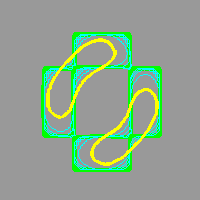
\includegraphics[width=0.22\textwidth]{images/demo/curvature_flow/curvature_flow5}	&
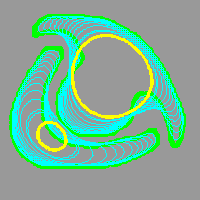
\includegraphics[width=0.22\textwidth]{images/demo/curvature_flow/curvature_flow6}	&
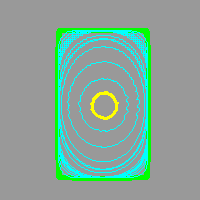
\includegraphics[width=0.22\textwidth]{images/demo/curvature_flow/curvature_flow7}	&
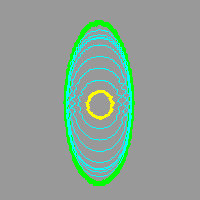
\includegraphics[width=0.22\textwidth]{images/demo/curvature_flow/curvature_flow8}
\end{tabular}
\caption[Motion by mean curvature.]{Example of motion by mean curvature. Initial curve is shown in green and the result after 500 iterations is shown in yellow. Intermediate stages of curve evolution are shown in cyan.}
\label{fig:mean_curvature_demo}
\end{figure}
For 3D applications, we have a closed surface instead of a curve. An area minimizing regularizer can be obtained by replacing the curvature term $\kappa$ in 2D by $H$ which is the sum of the principal curvatures of the surface in 3D \cite{caselles_minimal_surface}. However, unlike the 2D case, mean curvature motion is not the optimal area minimizing flow and there has been other models proposed in the literature \cite{caselles_minimal_surface,tannenbaum1997invariant}.

\subsection{Malladi-Sethian model}
The  above mentioned motion models are not really suitable for object segmentation, since neither (\ref{eq:const_speed}) or (\ref{eq:curvature_motion}) consider any information from the image. Malladi and Sethian \cite{malladi_sethian} introduced a flow based on the image model for object segmentation based on the gradient of the image. If $g(|\nabla f|)$ is a function which assumes a high value at the homogeneous portions of the image and significantly low value($\approx 0$) at the edges. One particular realization may be computed as $g=1/(1+|\nabla f|^q)$. With this definition, the curve motion equation is realized as:
\bea
\textbf{C}_t = g(|\nabla f|)(c_0+\kappa)\;\textbf{n}
\label{eq:malladi_sethian}
\eea
The function $g(.)$ acts as an edge indicator, by slowing down the speed of the snake when it approaches an edge, characterized by high gradient value. As before, the sign of the scalar $c_0$ dictates whether the snake moves outward or inward. The curvature based term imparts smoothness to the solution by disallowing irregular contour shapes.


\subsection{Geodesic Active Contour (GAC)}
Caselles et al.\cite{caselles_GAC} realized a drawback of Malladi's model which restricted its applicability in certain scenarios. This is because the function $g(.)$ does not stop the snake propagation at the edges, but merely slows it down. Therefore, if the edge strength is not significant enough, the propagating curve may not converge at the boundary but continue its motion and eventually collapse or diverge out.
\bea
\textbf{C}_t = g(|\nabla f|)(c_0+\kappa)\;\textbf{n}-\langle\nabla g,\textbf{n} \rangle \;\textbf{n}
\label{eq:GAC}
\eea
\begin{figure}[t]
\centering
\renewcommand{\tabcolsep}{0.05cm}
\begin{tabular}{@{}ccc@{}}
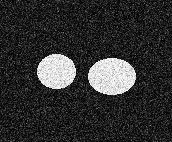
\includegraphics[width=0.3\textwidth]{images/demo/GAC/blobs_gaussian}	&
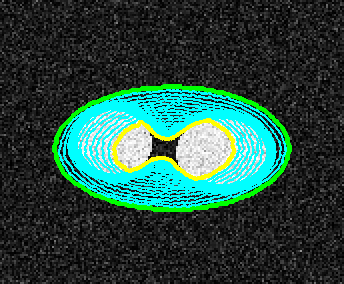
\includegraphics[width=0.3\textwidth]{images/demo/GAC/malladi_bad}	&
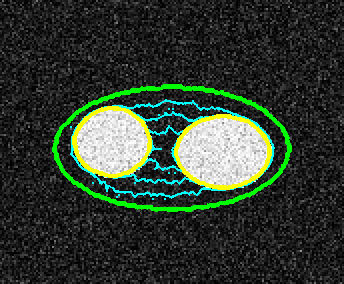
\includegraphics[width=0.3\textwidth]{images/demo/GAC/GAC_good}	\\
(a) original image & (b) Malladi-Sethian  & (c) GAC
\end{tabular}
\caption[GAC vs Malladi-Sethian model]{Segmentation performance of geodesic active contour model over Malladi-Sethian's method. The initial curve is shown in green and the final contour in yellow. Intermediate steps are shown in cyan.}
\label{fig:GACvsMalladi}
\end{figure}

The first part of (\ref{eq:GAC}) is similar to that of Malladi's model. The second term improves the evolution by incorporating a speed term which attracts the evolving curve towards the edge. This results in an additional component which halts the snake at the object boundaries. This is particularly helpful, since the function $g(.)$ does not stop the curve from leaking across the edges; it merely slows down the propagation speed. With the additional attraction term, the moving contour is attracted toward the edges and forces the curve to stop moving (see Fig.~\ref{fig:GACvsMalladi}).

 
This model can be interpreted as a flow that minimizes the geodesic curve length instead of the euclidean length, which makes it a geodesic length minimizing flow. For further detail, we refer the reader to the original paper\cite{caselles_GAC}.

\section{Implementation using level sets}
The previous subsection describes a few important active contour models. With a model already developed, the next challenge is that of implementation. This is where two subtypes of active contours emerge: \textit{parametric} and \textit{geometric}.

One way to implement the curve evolution equation (\ref{eq:curve_evolve_general}) is via discrete parametrization of the curve. The curve is represented by a set of finite number of contour pixels (or \textit{snaxels}), and the curve evolution is computed by explicitly calculating the deformation forces at these contour positions. Such algorithms fall under the category of parametric active contours and there has been significant research in this domain, involving both theoretical aspects
\cite{kwt_snakes,li_VFC,xu_GVF_journal,li_PIG,jacob2004efficient,bspline_snake,mishra2011decoupled} and practical applications\cite{leucocyte_dipti,ray2003merging,ray2002tracking,lesage2009review,zhu2014complete}. 

Parametric active contour methods are generally topology preserving, i.e., the topology of the evolving contour remains same during the motion. While this property may be desired in certain applications (e.g. tracking rigid objects), certain applications demand a methodology which is topology adaptive. For example, when multiple objects are present, one may wish to design an active contour model, which is capable of detecting each object despite starting from a single initialization. Unfortunately, parametric methods are incapable of handling changes in topology, unless specialized algorithms are developed to perform contour merging or splitting.

\subsection{Geometric active contour}
Osher and Sethian\cite{osher_sethian} proposed an implicit curve evolution method which makes the curve adaptive to the topology of the objects. This set of algorithms, popularly known as level set methods or geometric active contour methods represent the contour $\textbf{C}(\textbf{x},t)$  as the zero level set of a continuous functional $\phi$. With this representation, the curve evolution is obtained explicitly, by  deforming the functional $\phi$ instead of calculating the forces on the discretized contour positions. The function $\phi:\Omega\times\mathbb{R}^+\mapsto\mathbb{R}$ is defined such that the active contour is given by $\textbf{C}(\textbf{x},t)=\lbrace\textbf{x}:\phi(\textbf{x},t)=0\rbrace\;\forall t\in\mathbb{R}^+$. Furthermore, if $\Gamma_{in}\subseteq\Omega$ and $\Gamma_{out}\subseteq\Omega$ denote the regions inside and outside the zero level set of $\phi$, we have $\phi(\textbf{x}) \geq 0\; \forall \textbf{x}\in\Gamma_{in}$ and  $\phi(\textbf{x}) < 0\; \forall \textbf{x}\in\Gamma_{out}$.

The advantage of using the embedding functional $\phi$ is that all operations are carried out on $\phi$ and the evolving contour is represented by the zero level set of $\phi$. Using this implicit representation of the curve enjoys the benefit of topological adaptivity; the embedding function has natural ability of merging and splitting -- which subsequently allows the zero level set to merge and split without the use of specialized schemes. 

Naturally, the next question is how to modify (\ref{eq:curve_evolve_general}) so that the implicit motion can be accommodated? As it turns out, it is quite trivial to develop a relationship between the explicit motion model and the implicit model. Assuming that the curve motion equation is given by (\ref{eq:curve_evolve_general}), the explicit motion model is given by
\bea
\phi_t + \langle\textbf{C}_t,\nabla\phi \rangle = 0
\label{eq:explicit_motion_ls}
\eea
The outward normal vector and curvature are computed as
\bea
\textbf{n}&=&-\dfrac{\nabla\phi}{|\nabla\phi|}\\
\kappa&=&\text{div}\left(\dfrac{\nabla\phi}{|\nabla\phi|}\right)
\label{eq:normal_curvature_ls}
\eea
Derivation details are given in the Appendix. Now that we have obtained an equivalence between the implicit and explicit representations, we can modify the curve motion models in the level set framework. 

\begin{table}[bht]
\centering
\caption[Geometric Flow]{Equivalent geometric flow equations using level set representation.}
\begin{tabular}{c|c|c}
Motion model & Curve motion model & Geometric model \\
\hline \hline 
Constant speed motion & $\textbf{C}_t=c_0\, \textbf{n}$ & $\phi_t=c_0|\nabla
\phi|$ \\
Mean curvature motion & $\textbf{C}_t=\kappa\, \textbf{n}$ & $\phi_t=\text{div}\left(\dfrac{\nabla\phi}{|\nabla\phi|}\right)|\nabla
\phi|$ \\
Malladi-Sethian model & $\textbf{C}_t=g(.)\left(c_0+\kappa\right) \textbf{n}$ & $\phi_t=g(.)\left(c_0+\kappa\right)|\nabla
\phi|$ \\
Geodesic active contour & $g(.)\kappa\;\textbf{n}-\langle\nabla g,\|\textbf{n} \rangle \;\textbf{n}$ & $\phi_t= \text{div}\left(g(.)\dfrac{\nabla\phi}{|\nabla\phi|}\right)|\nabla\phi|$\\
\hline
\end{tabular}
\label{table:geometric_flow}
\end{table}
Explicit curve motion equation involving the embedding function is popularly known as \textit{geometric flow} equation. The benefit of the geometric model is its topological flexibility. Such models are very efficient in segmenting multiple objects and have been used for numerous applications in image analysis. Implementation of the geometric flow is performed by discretizing the function $\phi$ over an uniform grid and using tools from numerical methods to solve the partial differential equation. 

It is desirable that the embedding function is a differentiable function which is positive inside the zero level set and negative outside it. Also, since the zero level set of $\phi$ gives the position of the contour at each step of iteration, it is important to maintain the property of $\phi$ during the flow. This is performed by a process known as \textit{reinitialization} which allows $\phi$ to retain the properties of a geometric embedding function and  prevents instability. Several reinitialization techniques have been proposed in the literature including pde based methods and variational methods\cite{osher_sethian,caselles_geodesic,li_without_reinit_CVPR,li_DRLS}. 


While topology adaptability is a feature of geometric models which is unavailable with the parametric setup, one loses out in terms of computational time. While parametric models operate on a set of discrete points, the geometric models demand the entire functional $\phi$ to be updated at each interval. There has been concerted efforts to reduce the computational time of such methods which includes narrow band methods (where update is performed only at positions near the zero level sets), fast marching and multigrid methods\cite{malladi_sethian,papandreou2007multigrid,goldenberg2001fast,sethian1999fast,shi2008real}. 

\section{Variational active contours}

In the previous sections, we have described active contour models in a top down fashion. An equation for propagating the curve is first established and then implicit curve motion is obtained by using an embedding functional. Designing such models generally involve computing a suitable speed function $F$ (see eq. (\ref{eq:curve_evolve_general})). In many cases, it is convenient to design a solution by finding a suitable speed function or force function. This force function typically consists of a smoothness invoking part and an image based component which generally attracts the level set to the regions of high gradient in the image\cite{malladi_sethian,caselles_geodesic}. Consequently, such techniques are categorized as  \textit{edge based} techniques.

However, in certain applications, the object segmentation may be performed as a (possibly local) solution to a suitable optimization problem. A popular example is that of region based segmentation framework proposed by Mumford and Shah \cite{mumford_shah}. The authors introduced a segmentation methodology which attempts to cluster the image into sets of foreground and background pixels based on their gray level intensity.
The variational segmentation methodology can be mathematically stated as follows:
\bea
\phi^*&=&\underset{\phi}{\arg\!\min}\;\mathcal{E}(\phi) \label{eq:variational_ls_basic}
\\
\phi_t &=& -\nabla_{\phi}\;\mathcal{E}(\phi)
\label{eq:variational_grad_flow}
\eea
The zero level sets of the local minimizer $\phi^*$ of an energy functional $\mathcal{E}(\phi)$ corresponds to the detected object boundaries (eq. (\ref{eq:variational_ls_basic})). Generally, a gradient descent based algorithm is deployed to find the local minima of the functional and the solution is computed iteratively. The gradient descent equation (\ref{eq:variational_grad_flow}) corresponds to the curve propagation partial differential equation (similar to (\ref{eq:curve_evolve_general})) for the variational scheme which is derived using variational calculus\cite{calc_of_var}. This equation is often referred to as \textit{variational flow equation} or \textit{gradient flow equation}. 

The variational problem requires specification of the energy functional $\mathcal{E}(\phi)$. Traditionally, an energy function consists of two terms-- a regularization term $\mathcal{E}_r(\phi)$ which generates smooth solution and another data term $\mathcal{E}_d(\phi,f(\textbf{x}))$ which usually incorporates image based features for segmentation \cite{zhao_variational,chan_vese,bernard_splinedCV,lankton_localCV}. In addition, segmentation performance can be significantly improved by incorporating prior information about the object shape . Variational formulations provide an elegant way to introduce such priors in form of an additive energy term and may be introduced both as a hard prior\cite{chan_LS_shape,cremers2007review,foulonneau2006affine,gooya2008variational} or a soft prior\cite{nain2004vessel}.

\subsection{Variational contour regularization}
Here we discuss two popularly used energy functionals used for the purpose of obtaining a smooth active contour. One way to regularize the shape of the contour is by restricting its total length. This is performed by minimizing eq. (\ref{eq:length_reg}), and the gradient flow equation is obtained by deriving the Euler-Lagrange equation and using gradient descent for local solution. This is shown in eq. (\ref{eq:length_reg_flow}).
\bea
\mathcal{E}_{r}^{(1)}&=&\int_{\Omega}|\nabla H(\phi)|d\textbf{x} \label{eq:length_reg} \\
\phi_t&=&\text{div}\left(\dfrac{\nabla \phi}{|\nabla \phi|}\right)\delta\left(\phi\right)
\label{eq:length_reg_flow}
\eea
Here $H(.)$ is the Heaviside function defined such that $H(y)=1\; \forall y>=0$ and $H(y)=0$ otherwise. In otherwise, the Heaviside function serves as an indicator function for the area inside the zero level set of $\phi$. $\delta(.)$ is the Dirac delta function. Since the Heaviside function is not differentiable, for practical purposes the following regularized versions of the Heaviside and Dirac functions are used\cite{chan_vese}. 
\bea
\heav(q)&=& \dfrac{1}{2}\left(1+\dfrac{2}{\pi}\tan^{-1}\left(\dfrac{q}{\epsilon}\right)\right) \label{eq:heav_relax} \\
\dirac(q) &=& \dfrac{d}{dq}\heav(q) \label{eq:dirac_relax}
\eea
Analyzing eq. (\ref{eq:length_reg}), it is not difficult to comprehend that the right hand side of the equation corresponds to the total length of the zero level set of $\phi$. Therefore, eq. (\ref{eq:length_reg_flow}) represents the curve evolution equation such that the length of the curve is locally minimized. One can find a similarity between the length shortening gradient flow (\ref{eq:length_reg_flow}) and the mean curvature motion in (\ref{eq:curvature_motion}), where the expressions differ by the multiplicative terms. In fact, if only a narrow band around the zero level contour is considered, one can find that both these formulations lead to almost identical solutions that regularizes the curve via length minimization.


Another regularization popularly  used for getting a smooth solution is obtained by minimizing the total area inside the contour. The area minimizing smoothing functional and the corresponding gradient flow equation are computed as follows:
\bea
\mathcal{E}_{r}^{(2)}&=&\int_{\Omega}\heav(\phi)d\textbf{x} \label{eq:area_reg} \\
\phi_t&=&-\dirac(\phi) \label{eq:area_reg_flow}
\eea
The regularizing energy functional contributes only to the smoothness of the solution. The regularizers are generally not dependent on image features. however, to perform segmentation, one needs to engineer a suitable data term that incorporates image based information (such as intensity, edge strength, texture etc.) to drive the level sets toward the desired object boundaries.
 
\subsection{Chan-Vese's segmentation model}
Chan and Vese\cite{chan_vese} proposed a level set formulation to minimize the Mumford Shah functional \cite{mumford_shah} for segmentation. The Chan-Vese framework models the image as a set of constant illumination regions and performs a two-class segmentation by computing the optimal partition which satisfies the constant illumination constraint. The authors also propose a multi-phase variant \cite{vese_multiphase} of their approach to perform multi class grouping. 

The piecewise constant model of Chan-Vese\cite{chan_vese}  models the object foreground and background by the scalars $c_1$ and $c_2$. In a level set framework, the Chan-Vese energy functional $\mathcal{E}_d=\mathcal{E}_{CV}$ is written as follows:
\bea
\mathcal{E}_{CV}(\phi,c_1,c_2)= \int_{\Omega}|f(\textbf{x})-c_1|^2H(\phi) d\textbf{x} 
						   +\int_{\Omega}|f(\textbf{x})-c_2|^2 \left(1-H(\phi)\right) d\textbf{x}  
\label{eq:chan_vese}
\eea
Here $f(\textbf{x})$ is the image defined over the domain $\Omega$. The $\phi$ that locally minimizes (\ref{eq:chan_vese}) creates segments in a manner such that the foreground and background are best approximated by the intensity levels $c_1$ and $c_2$.


The (local) minima of (\ref{eq:chan_vese}) is obtained using alternate minimization. In the first step, the optimal values of the scalars $c_1,c_2$ are obtained as follows:
\bea
c_1^*,c_2^*& = &\underset{c_1,c_2}{\arg\!\min}\, \mathcal{E}_d(\phi,c_1,c_2) \\
\phi^* & = & \underset{\phi}{\arg\!\min}\, \mathcal{E}_d(\phi,c_1^*,c_2^*)
\eea
The solution for $c_1^*\,\text{and} c_2^*$ is obtained in closed form as 
\bea
c_1^* = \dfrac{\int f(\textbf{x})\heav(\phi)d\textbf{x}}{\int \heav(\phi)d\textbf{x}},\;
c_2^* = \dfrac{\int f(\textbf{x})\left(1-\heav(\phi)\right)d\textbf{x}}{\int \left(1-\heav(\phi)\right)d\textbf{x}}
\label{eq:cv_scalars}
\eea
With these updated values, the local optima for the embedding function $\phi$ is computed by iteratively solving the following gradient flow equation.
\bea
\phi_t = \left[-(f(\textbf{x})-c_1^*)^2+(f(\textbf{x})-c_2^*)^2\right]\dirac(\phi)
\label{eq:cv_flow}
\eea

In addition to (\ref{eq:cv_flow}), a regularizer term as in (\ref{eq:length_reg_flow}) is also added to obtain smooth boundaries. The above mentioned model is particularly useful when the object edges are not prominent or the edges are blurred.  Also, region based methodologies exhibit significant performance benefits for noisy images where the accuracy of the edge map is sacrificed due to noise. 


\section{Edge based vs. region based models}

\subsection{Synthetic examples}
Fig.~\ref{fig:GACvsCV} compares the performance of Geodesic Active Contour \cite{caselles_geodesic} algorithm which is an edge based framework versus the region based segmentation technique due to Chan and Vese\cite{chan_vese}. To demonstrate the properties of each algorithm, we simulate four images. The first image is that of a disc (Fig.~\ref{fig:GACvsCV}(a), row 1) with homogeneous intensity level. This image has uniform illumination and the edges are well defined. Therefore, such an image is a good candidate for segmentation with either edge based or region based approaches. It is observed that both the algorithms perform almost identically in this case.
\begin{figure}[tb]
\centering
\renewcommand{\tabcolsep}{0.05cm}
\begin{tabular}{@{}ccc@{}}
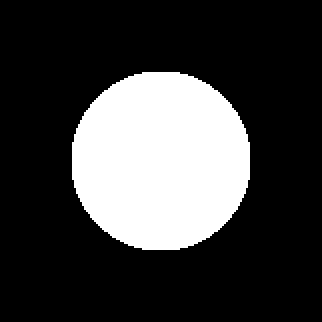
\includegraphics[width=0.3\textwidth]{images/demo/GACvsCV/disk}	&
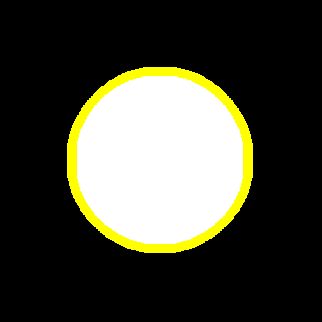
\includegraphics[height=0.3\textwidth]{images/demo/GACvsCV/GAC_disc}	&
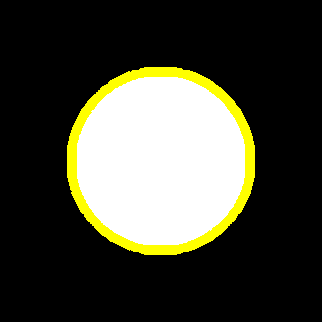
\includegraphics[height=0.3\textwidth]{images/demo/GACvsCV/CV_disc}	\\
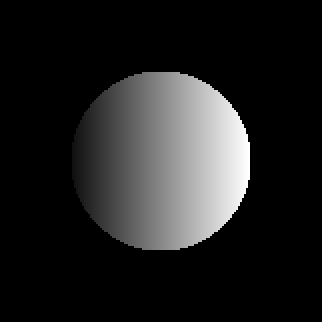
\includegraphics[width=0.3\textwidth]{images/demo/GACvsCV/inhom}	&
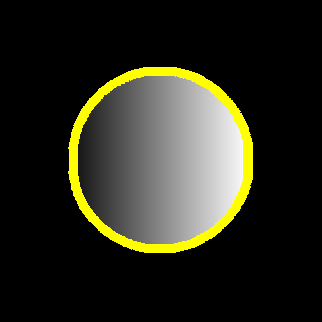
\includegraphics[height=0.3\textwidth]{images/demo/GACvsCV/GAC_inhom}	&
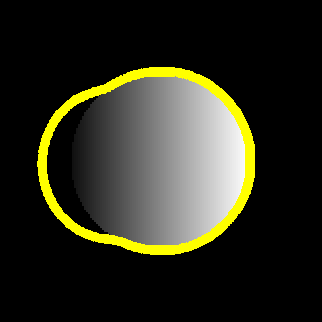
\includegraphics[height=0.3\textwidth]{images/demo/GACvsCV/CV_inhom}	\\
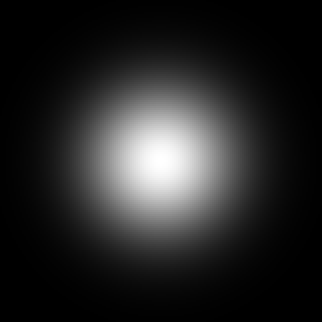
\includegraphics[width=0.3\textwidth]{images/demo/GACvsCV/gauss}	&
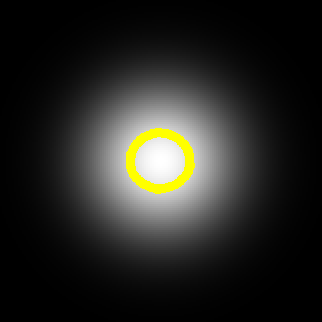
\includegraphics[height=0.3\textwidth]{images/demo/GACvsCV/GAC_gauss}	&
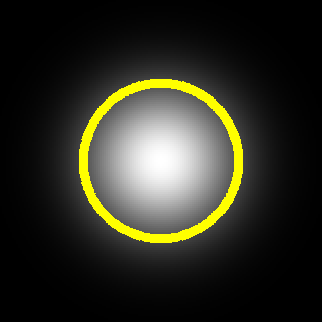
\includegraphics[height=0.3\textwidth]{images/demo/GACvsCV/CV_gauss}	\\
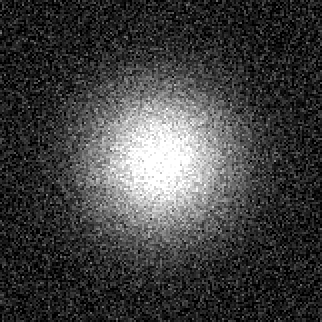
\includegraphics[width=0.3\textwidth]{images/demo/GACvsCV/gauss_noisy}	&
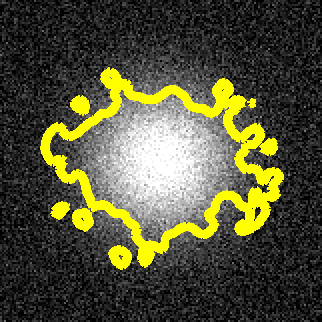
\includegraphics[height=0.3\textwidth]{images/demo/GACvsCV/GAC_gauss_noisy}	&
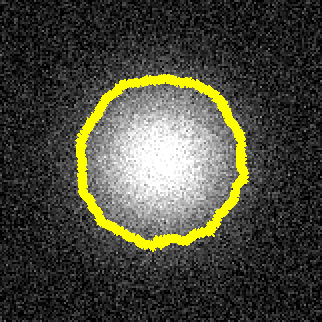
\includegraphics[height=0.3\textwidth]{images/demo/GACvsCV/CV_gauss_noisy}	\\
(a) simulated image & (b) GAC\cite{caselles_GAC} & (c) Chan-Vese\cite{chan_vese}
\end{tabular}
\caption[Edge based model vs region based model]{(a)Simulated images. (b)Segmentation performance of (GAC\cite{caselles_GAC}) and (c) Results via (Chan-Vese\cite{chan_vese}). The final result is shown by the yellow contour.}
\label{fig:GACvsCV}
\end{figure}

The second image (Fig.~\ref{fig:GACvsCV}(a), row 2) is that of a disc with non uniform intensity. However, the object edges are still relatively well defined. As a result, almost perfect segmentation is obtained using the GAC model. However, Chan and Vese's algorithm is incapable of handling intensity inhomogeneity. This is a significant deficiency of this method and it would be dealt with substantial rigor in the next chapter. The piecewise constant illumination model of Chan-Vese fails to produce correct segmentation, and we observe false positive in (Fig.~\ref{fig:GACvsCV}(c), row 2).

In the third example (Fig.~\ref{fig:GACvsCV}(a), row 3), the edges of the disc are blurred by smoothing it with a Gaussian filter. As expected, the edge based algorithm fails to identify the proper object boundary, whereas the region based technique performs significantly better.

Finally, the fourth image (Fig.~\ref{fig:GACvsCV}(a), row 4) is simulated by adding zero mean Gaussian noise to the blurry disc image. We observe that region based segmentation is particularly robust against additive noise and the segmentation performance is not degraded significantly. On the other hand, GAC model faces difficulties both due to blurred edges as well as signal noise.

\subsection{Real examples}
\begin{figure}[t]
\centering
\renewcommand{\tabcolsep}{0.05cm}
\begin{tabular}{@{}ccc@{}}
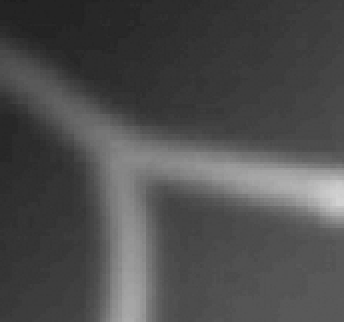
\includegraphics[width=0.3\textwidth]{images/L2S_compare/orig_1}	&
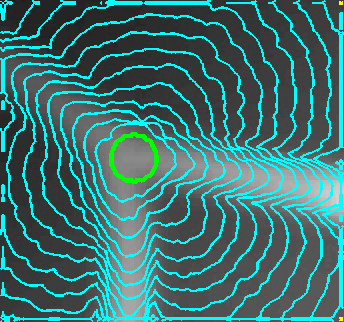
\includegraphics[width=0.3\textwidth]{images/L2S_compare/GAC_1}	&
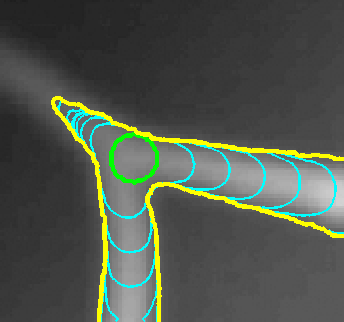
\includegraphics[width=0.3\textwidth]{images/L2S_compare/CV_1}	\\
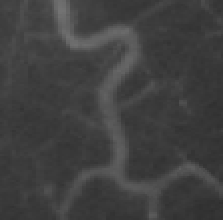
\includegraphics[width=0.3\textwidth]{images/L2S_compare/orig_4}	&
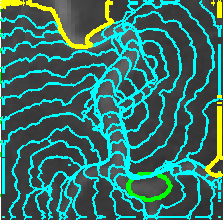
\includegraphics[width=0.3\textwidth]{images/L2S_compare/GAC_4}	&
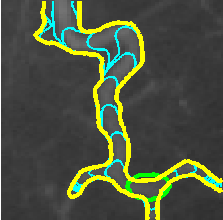
\includegraphics[width=0.3\textwidth]{images/L2S_compare/CV_4}	\\
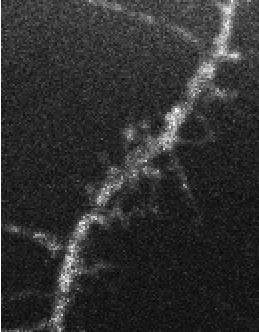
\includegraphics[width=0.3\textwidth]{images/L2S_compare/orig_5}	&
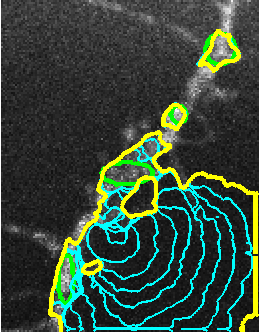
\includegraphics[width=0.3\textwidth]{images/L2S_compare/GAC_5}	&
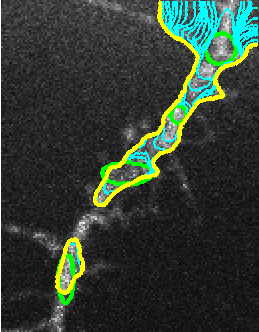
\includegraphics[width=0.3\textwidth]{images/L2S_compare/CV_5}	\\
(a) original image & (b) GAC & (c) Chan Vese
\end{tabular}
\caption[Geometric Snakes: negative examples]{Cases of improper segmentation using geometric contours. (a) Five images including simulated and real examples with varying illumination and weak edges. (b) Shows segmentation using geodesic active contour and (c) Shows segmentation due to Chan-Vese's method. The initial contour is plotted in green and the final contour in yellow. Intermediate steps of curve evolution are shown in cyan. This figure is best viewed in color.}
\label{fig:ls_compare}
\end{figure}
In Fig.~\ref{fig:ls_compare}, comparitive study of segmentation performance of geodesic active contour model and Chan-Vese's technique is presented on a set of real images consisting of vascular structures (neurons and retinal blood vessels) imaged using fluorescence microscope. Fluorescence microscopy images are often plagued by noise, inhomogeneous intensity and low contrast which leads to poor edge strength. 
As a result, we find that neither \cite{caselles_geodesic} nor \cite{chan_vese} is perfectly suitable for segmentation under such conditions. Segmentation error is caused either due to the curve leakage phenomenon (Fig.~\ref{fig:ls_compare}(b)) or under segmentation (Fig.~\ref{fig:ls_compare}(c)). In the following chapter, we attempt to design a generic segmentation algorithm which is tolerant to the commonly occurring artifacts in fluorescence microscopy.

\section{Discussion} 
In this chapter we have provided a broad overview of geometric active contours. Geometric contours are topology adaptive which makes them particularly attractive choice for segmentation. The segmentation model is either described in terms of explicit curve motion equation (\ref{eq:curve_evolve_n&t}) and then implemented by implicit representation of the contour as the zero level curve of an embedding functional (\ref{eq:explicit_motion_ls}). Another popular way to describe the segmentation process is via variational formulation which involves minimization of a suitable energy functional using variational calculus. The gradient flow equation (\ref{eq:variational_grad_flow}) is derived using gradient descent technique for computing the local minima of the functional. In either case, segmentation is performed by iteratively propagating the zero level set of the embedding function on a discrete grid borrowing tools from numerical mathematics.

Both formulations are widely used in the community and they enjoy their own sets of benefits. While curvature flow equations are often easy to conceptualize (e.g. equavalent to physical curve motion models such as wave propagation), variational models have gained popularity because of the flexibility to add further constraints in the solution in terms of shape prior. We also showed that in many cases it is possible to draw an analogy between the curve flow equations derived from the two techniques and in a majority of cases the results are quite comparable.

We then presented a comparison between edge based and region based methods for segmentation. It is shown that edge based models are more suitable for clean signals with strong edge response. Furthermore, such models are less susceptible to error if the object gray value is non homogeneous. Region based methods, on the other hand, are more robust to noise and do not depend particularly on the edge strength of the signal. However, it was demonstrated that the performance can degrade significantly in presence of intensity inhomogeneity. 

In the next chapter we focus our attention on segmenting vascular structures from 2D fluorescence microscopy images. As we have discussed briefly, fluorescence microscopy imagery are charecterized by poor contrast and varyinng intensity levels of the object.  This restricts the performance of the popular traditional geometric active contour models. This motivates us to develop a geometric segmentation model which is capable of handling noise and contrast fluctuations in the images.

